\section{Medición de coeficiente de absorción de materiales}
Como actividad extra del proyecto, se realizó el análisis del coeficiente de absorción sonora de una muestra de madera ranurada con lana mineral y lana de vidrio. (ver figura \ref{fig: materiales medicion coef abs})
%insertar imágenes de los materiales
\begin{figure}[H]
    \centering
    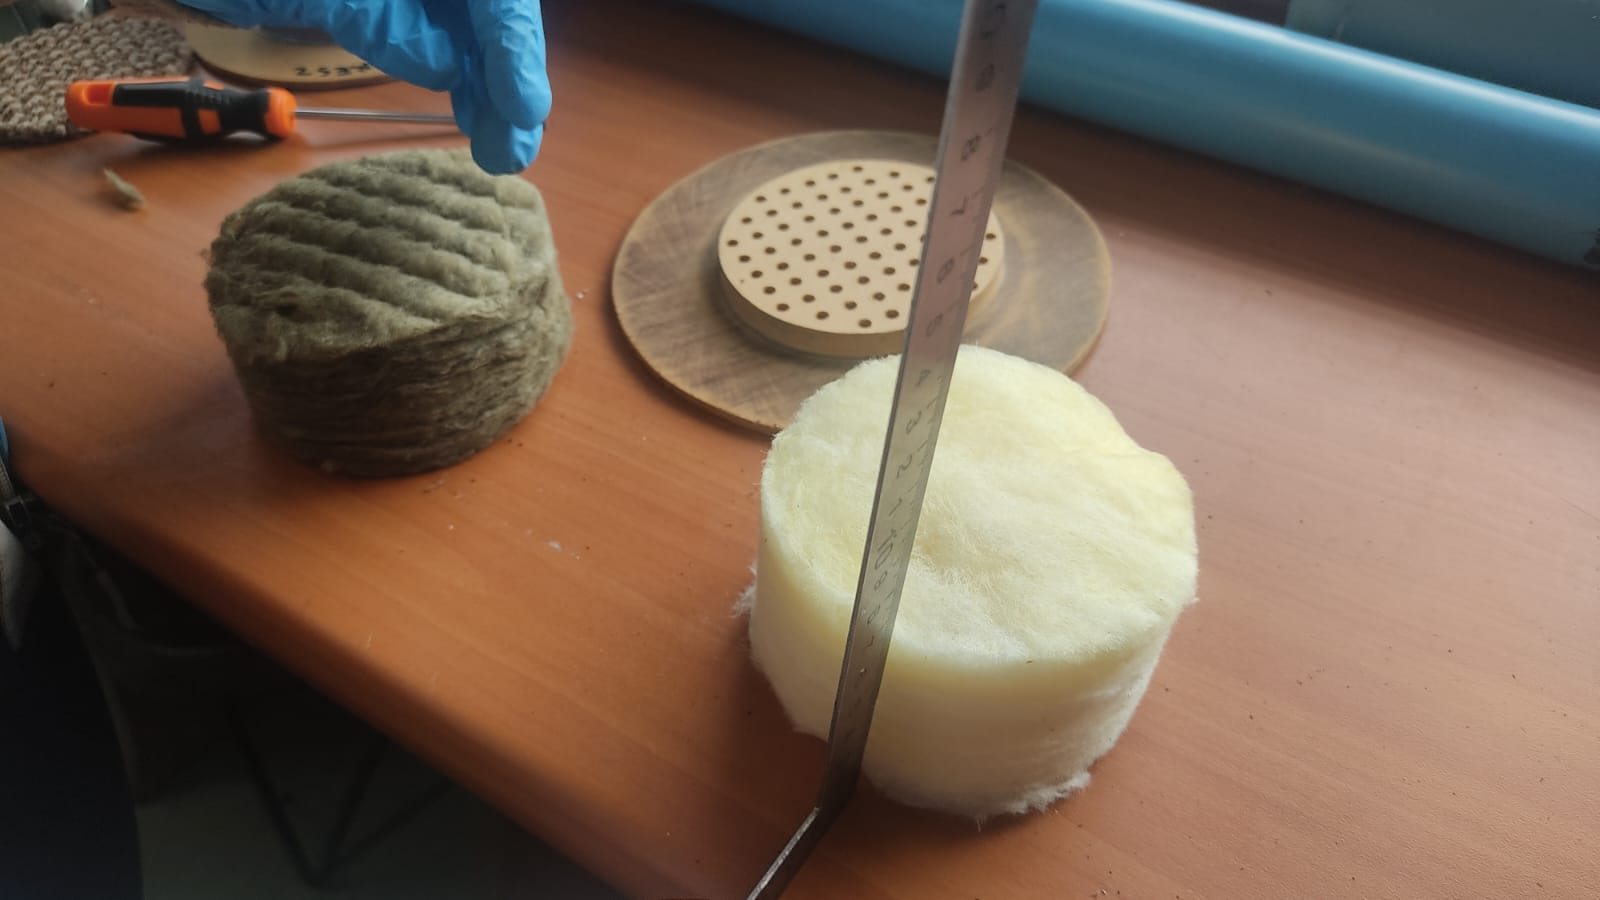
\includegraphics[width=8cm]{Imagenes/Medición abs/materiales.jpeg}
    \caption{Imágenes de materiales a medir}
    \label{fig: materiales medicion coef abs}
\end{figure}

La madera contaba con ranuras de diámetro de $5$mm y una distancia de $10$ mm entre ellas como lo indica la figura \ref{fig: madera medida}
%insertar imagen del material medido
\begin{figure}[H]
    \centering
    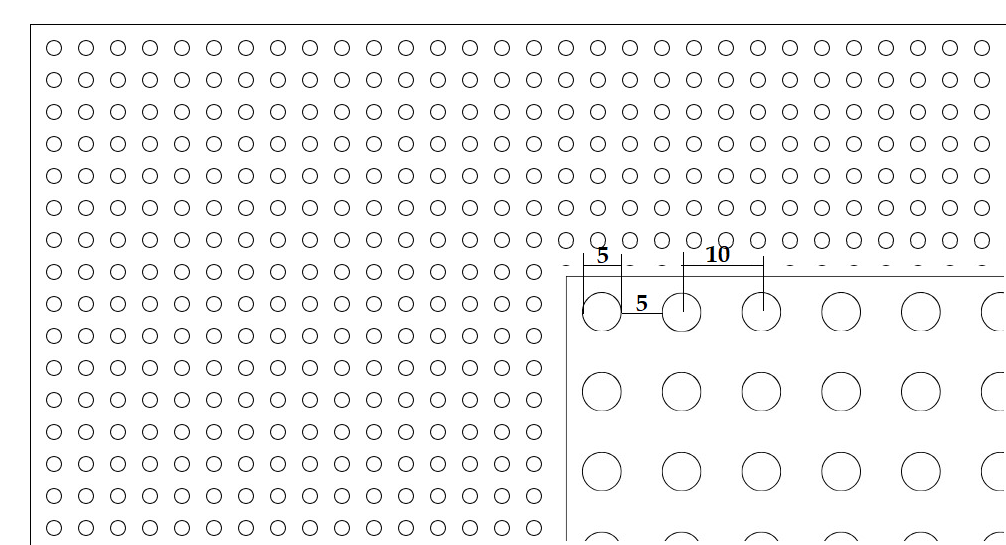
\includegraphics[width=8cm]{Imagenes/Medición abs/MATERIAL.png}
    \caption{Imagen de la madera ranurada medida}
    \label{fig: madera medida}
\end{figure}

Para realizar las mediciones se utilizó un tubo de impedancia con una muestra de cada materiales, combinando primero la madera con lana mineral sin plenum y un plenum de $2$ cm, y lo mismo con la lana de vidrio.\\
A raíz de las mediciones en el tubo se obtuvo el factor de reflexión, del cual se calculó el coeficiente de absorción de cada combinación a través de la fórmula \ref{eq: alpha} indicada en el anexo. Los coeficientes obtenidos se pueden observar en la tabla \ref{tab: coef de abs medidos} y en la figura \ref{fig: grafico de coef abs de lana mineral} y \ref{fig: grafico de coef abs de lana de vidrio}
%añadir grafico de coeficientes
\begin{table}[H]
    \centering
    \caption{coeficiente de absorción de los materiales}
    \label{tab: coef de abs medidos}
    \begin{tabular}{ll|llll|}
    \cline{3-6}
     &  & \multicolumn{4}{l|}{\textbf{Madera 5/10}} \\ \cline{3-6} 
     &  & \multicolumn{2}{l|}{Lana mineral $5$ cm} & \multicolumn{2}{l|}{Lana de vidrio $6$ cm} \\ \cline{2-6} 
    \multicolumn{1}{l|}{} & Plenum & \multicolumn{1}{l|}{\cellcolor[HTML]{8784C7}$0$ mm} & \multicolumn{1}{l|}{\cellcolor[HTML]{AD84C6}$200$ mm} & \multicolumn{1}{l|}{\cellcolor[HTML]{5D739A}$0$ mm} & \cellcolor[HTML]{6997AF}$200$ mm \\ \hline
    \multicolumn{1}{|l|}{} & $250$ & \multicolumn{1}{l|}{$0.44$} & \multicolumn{1}{l|}{$0.57$} & \multicolumn{1}{l|}{$0.48$} & $0.56$ \\ \cline{2-6} 
    \multicolumn{1}{|l|}{} & $315$ & \multicolumn{1}{l|}{$0.54$} & \multicolumn{1}{l|}{$0.69$} & \multicolumn{1}{l|}{$0.59$} & $0.66$ \\ \cline{2-6} 
    \multicolumn{1}{|l|}{} & $400$ & \multicolumn{1}{l|}{$0.73$} & \multicolumn{1}{l|}{$0.89$} & \multicolumn{1}{l|}{$0.78$} & $0.83$ \\ \cline{2-6} 
    \multicolumn{1}{|l|}{} & $500$ & \multicolumn{1}{l|}{$0.89$} & \multicolumn{1}{l|}{$0.97$} & \multicolumn{1}{l|}{$0.92$} & $0.95$ \\ \cline{2-6} 
    \multicolumn{1}{|l|}{} & $630$ & \multicolumn{1}{l|}{$0.99$} & \multicolumn{1}{l|}{$0.93$} & \multicolumn{1}{l|}{$0.94$} & $0.92$ \\ \cline{2-6} 
    \multicolumn{1}{|l|}{} & $800$ & \multicolumn{1}{l|}{$0.92$} & \multicolumn{1}{l|}{$0.77$} & \multicolumn{1}{l|}{$0.78$} & $0.77$ \\ \cline{2-6} 
    \multicolumn{1}{|l|}{} & $1000$ & \multicolumn{1}{l|}{$0.75$} & \multicolumn{1}{l|}{$0.61$} & \multicolumn{1}{l|}{$0.59$} & $0.60$ \\ \cline{2-6} 
    \multicolumn{1}{|l|}{} & $1250$ & \multicolumn{1}{l|}{$0.60$} & \multicolumn{1}{l|}{$0.52$} & \multicolumn{1}{l|}{$0.48$} & $0.50$ \\ \cline{2-6} 
    \multicolumn{1}{|l|}{} & $1600$ & \multicolumn{1}{l|}{$0.49$} & \multicolumn{1}{l|}{$0.49$} & \multicolumn{1}{l|}{$0.43$} & $0.47$ \\ \cline{2-6} 
    \multicolumn{1}{|l|}{\multirow{-10}{*}{\rotatebox{90}{Frecuencias Hz}}} & $2000$ & \multicolumn{1}{l|}{$0.52$} & \multicolumn{1}{l|}{$0.51$} & \multicolumn{1}{l|}{$0.42$} & $0.47$ \\ \hline
    \multicolumn{1}{l|}{} & $\alpha_{\omega}$ & \multicolumn{1}{l|}{$0.60$} & \multicolumn{1}{l|}{$0.60$} & \multicolumn{1}{l|}{$0.50$} & $0.55$ \\ \cline{2-6} 
    \end{tabular}
\end{table}

\begin{figure}[H]
    \centering 
    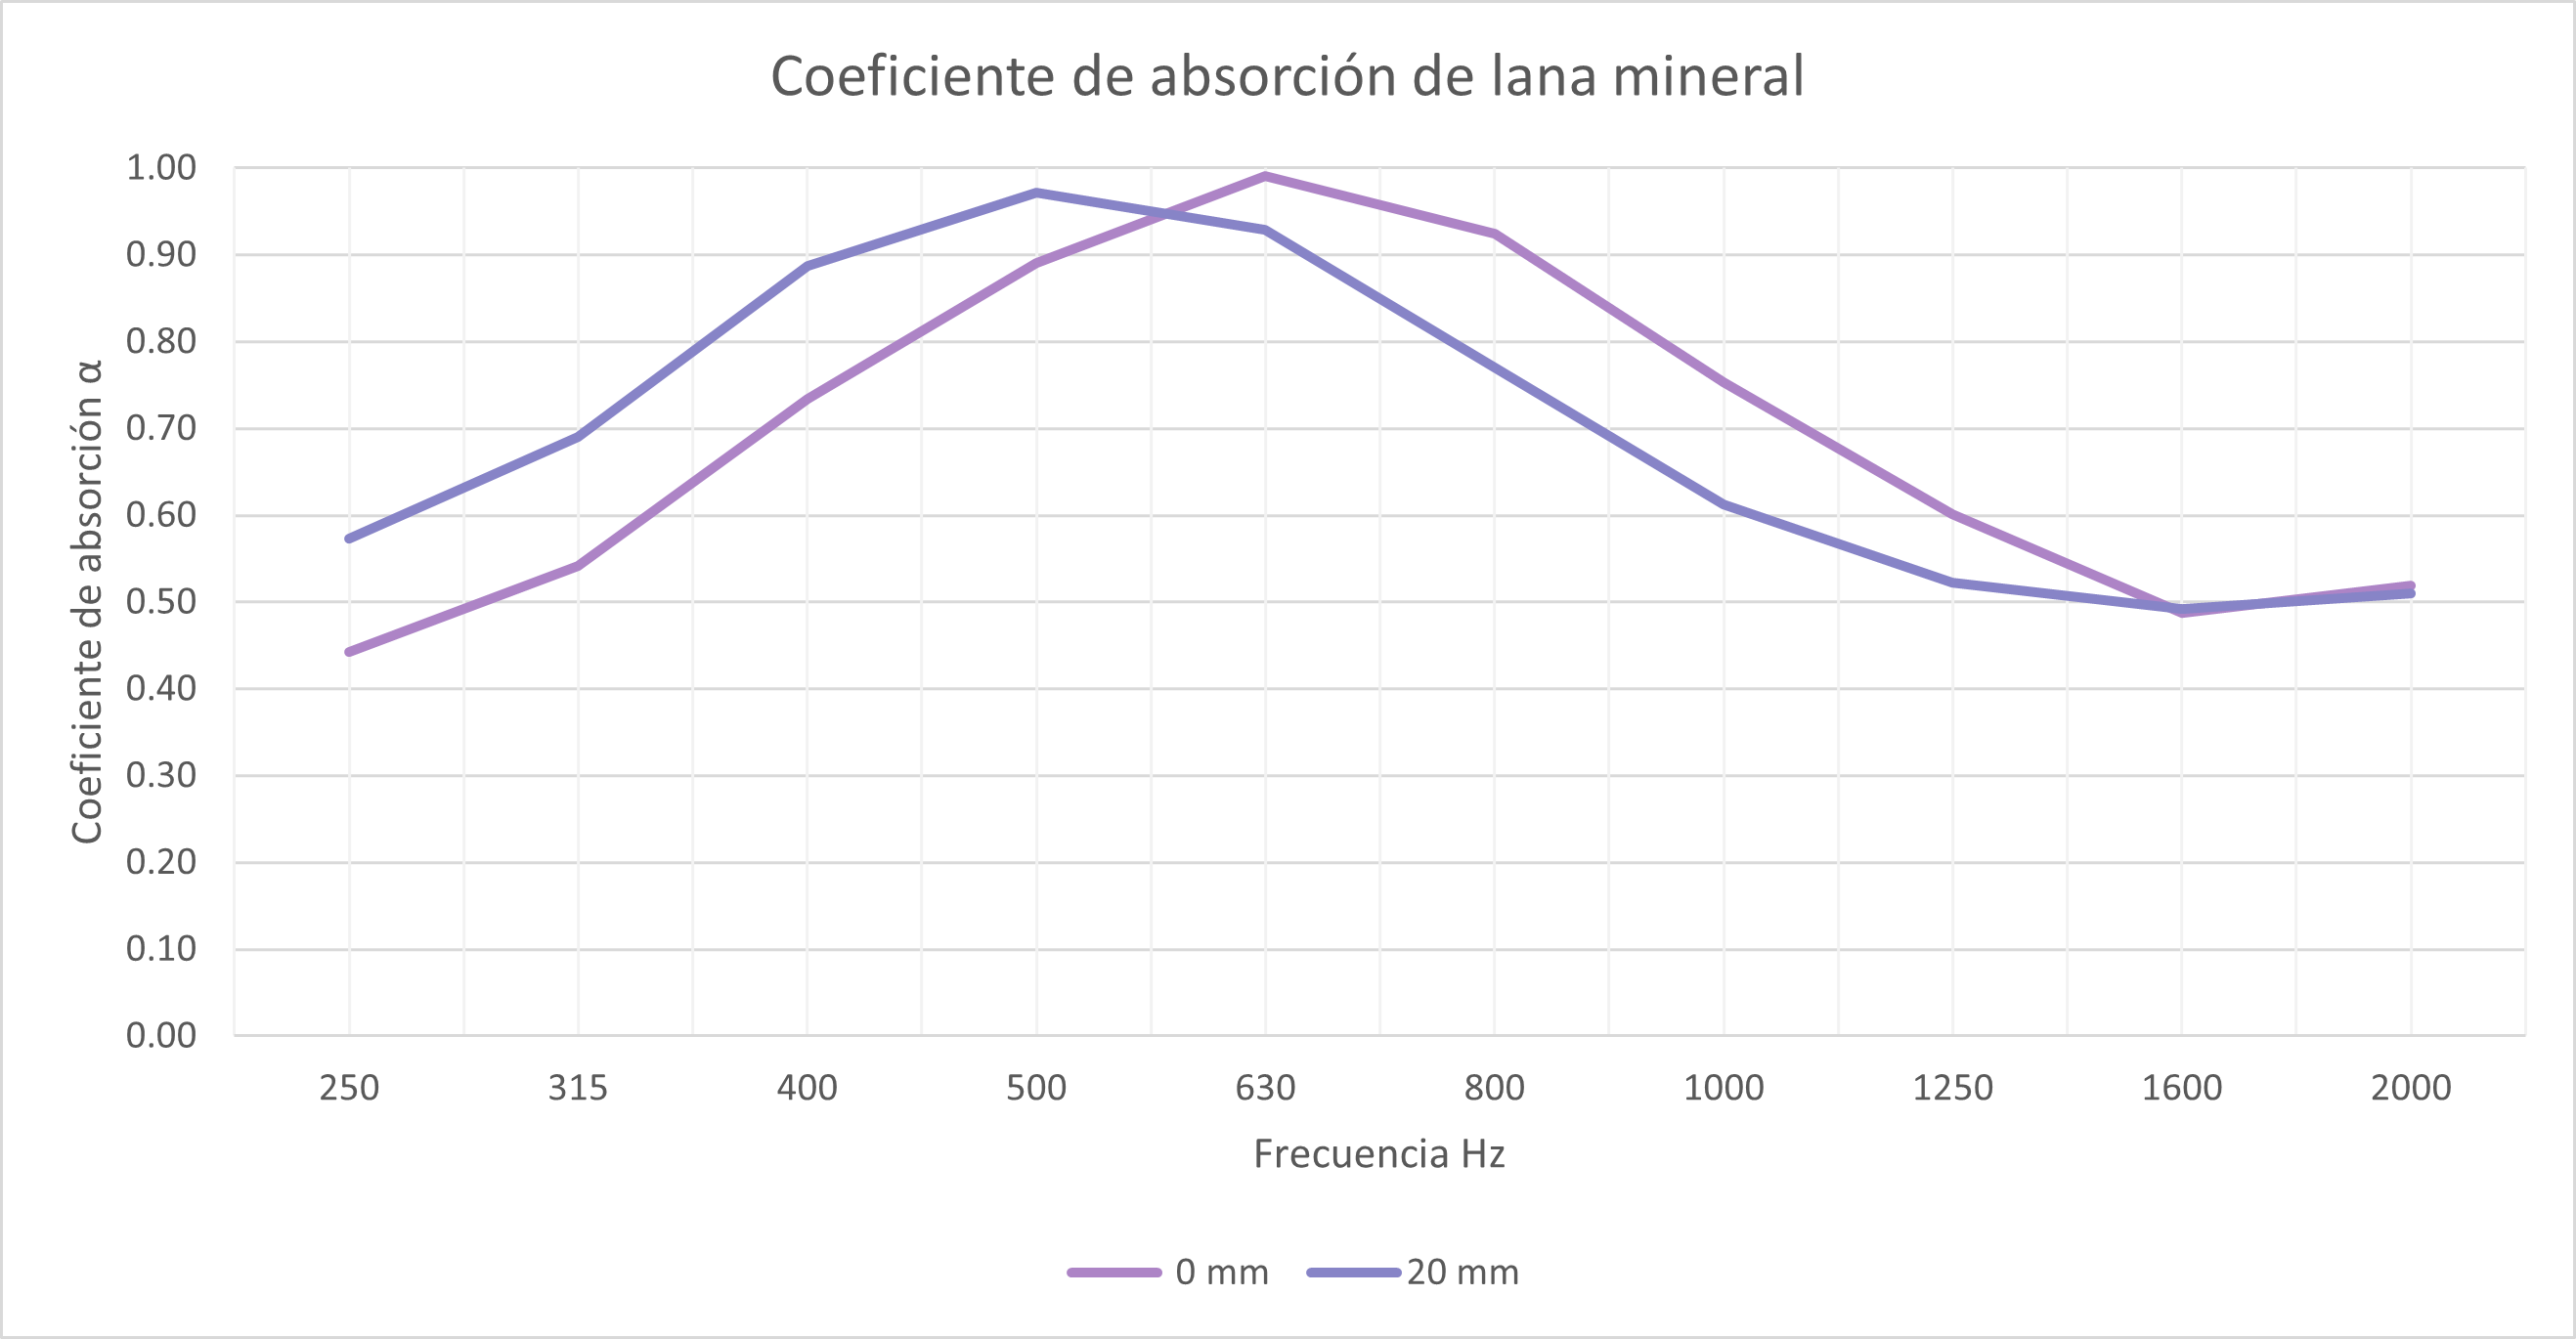
\includegraphics[width=10cm]{Imagenes/Medición abs/Grafico coef.abs LanaMineral.png}
    \caption{Gráfico de coeficiente de absorción de madera ranurada con lana mineral con distinto plenum}
    \label{fig: grafico de coef abs de lana mineral}
\end{figure}

\begin{figure}[H]
    \centering 
    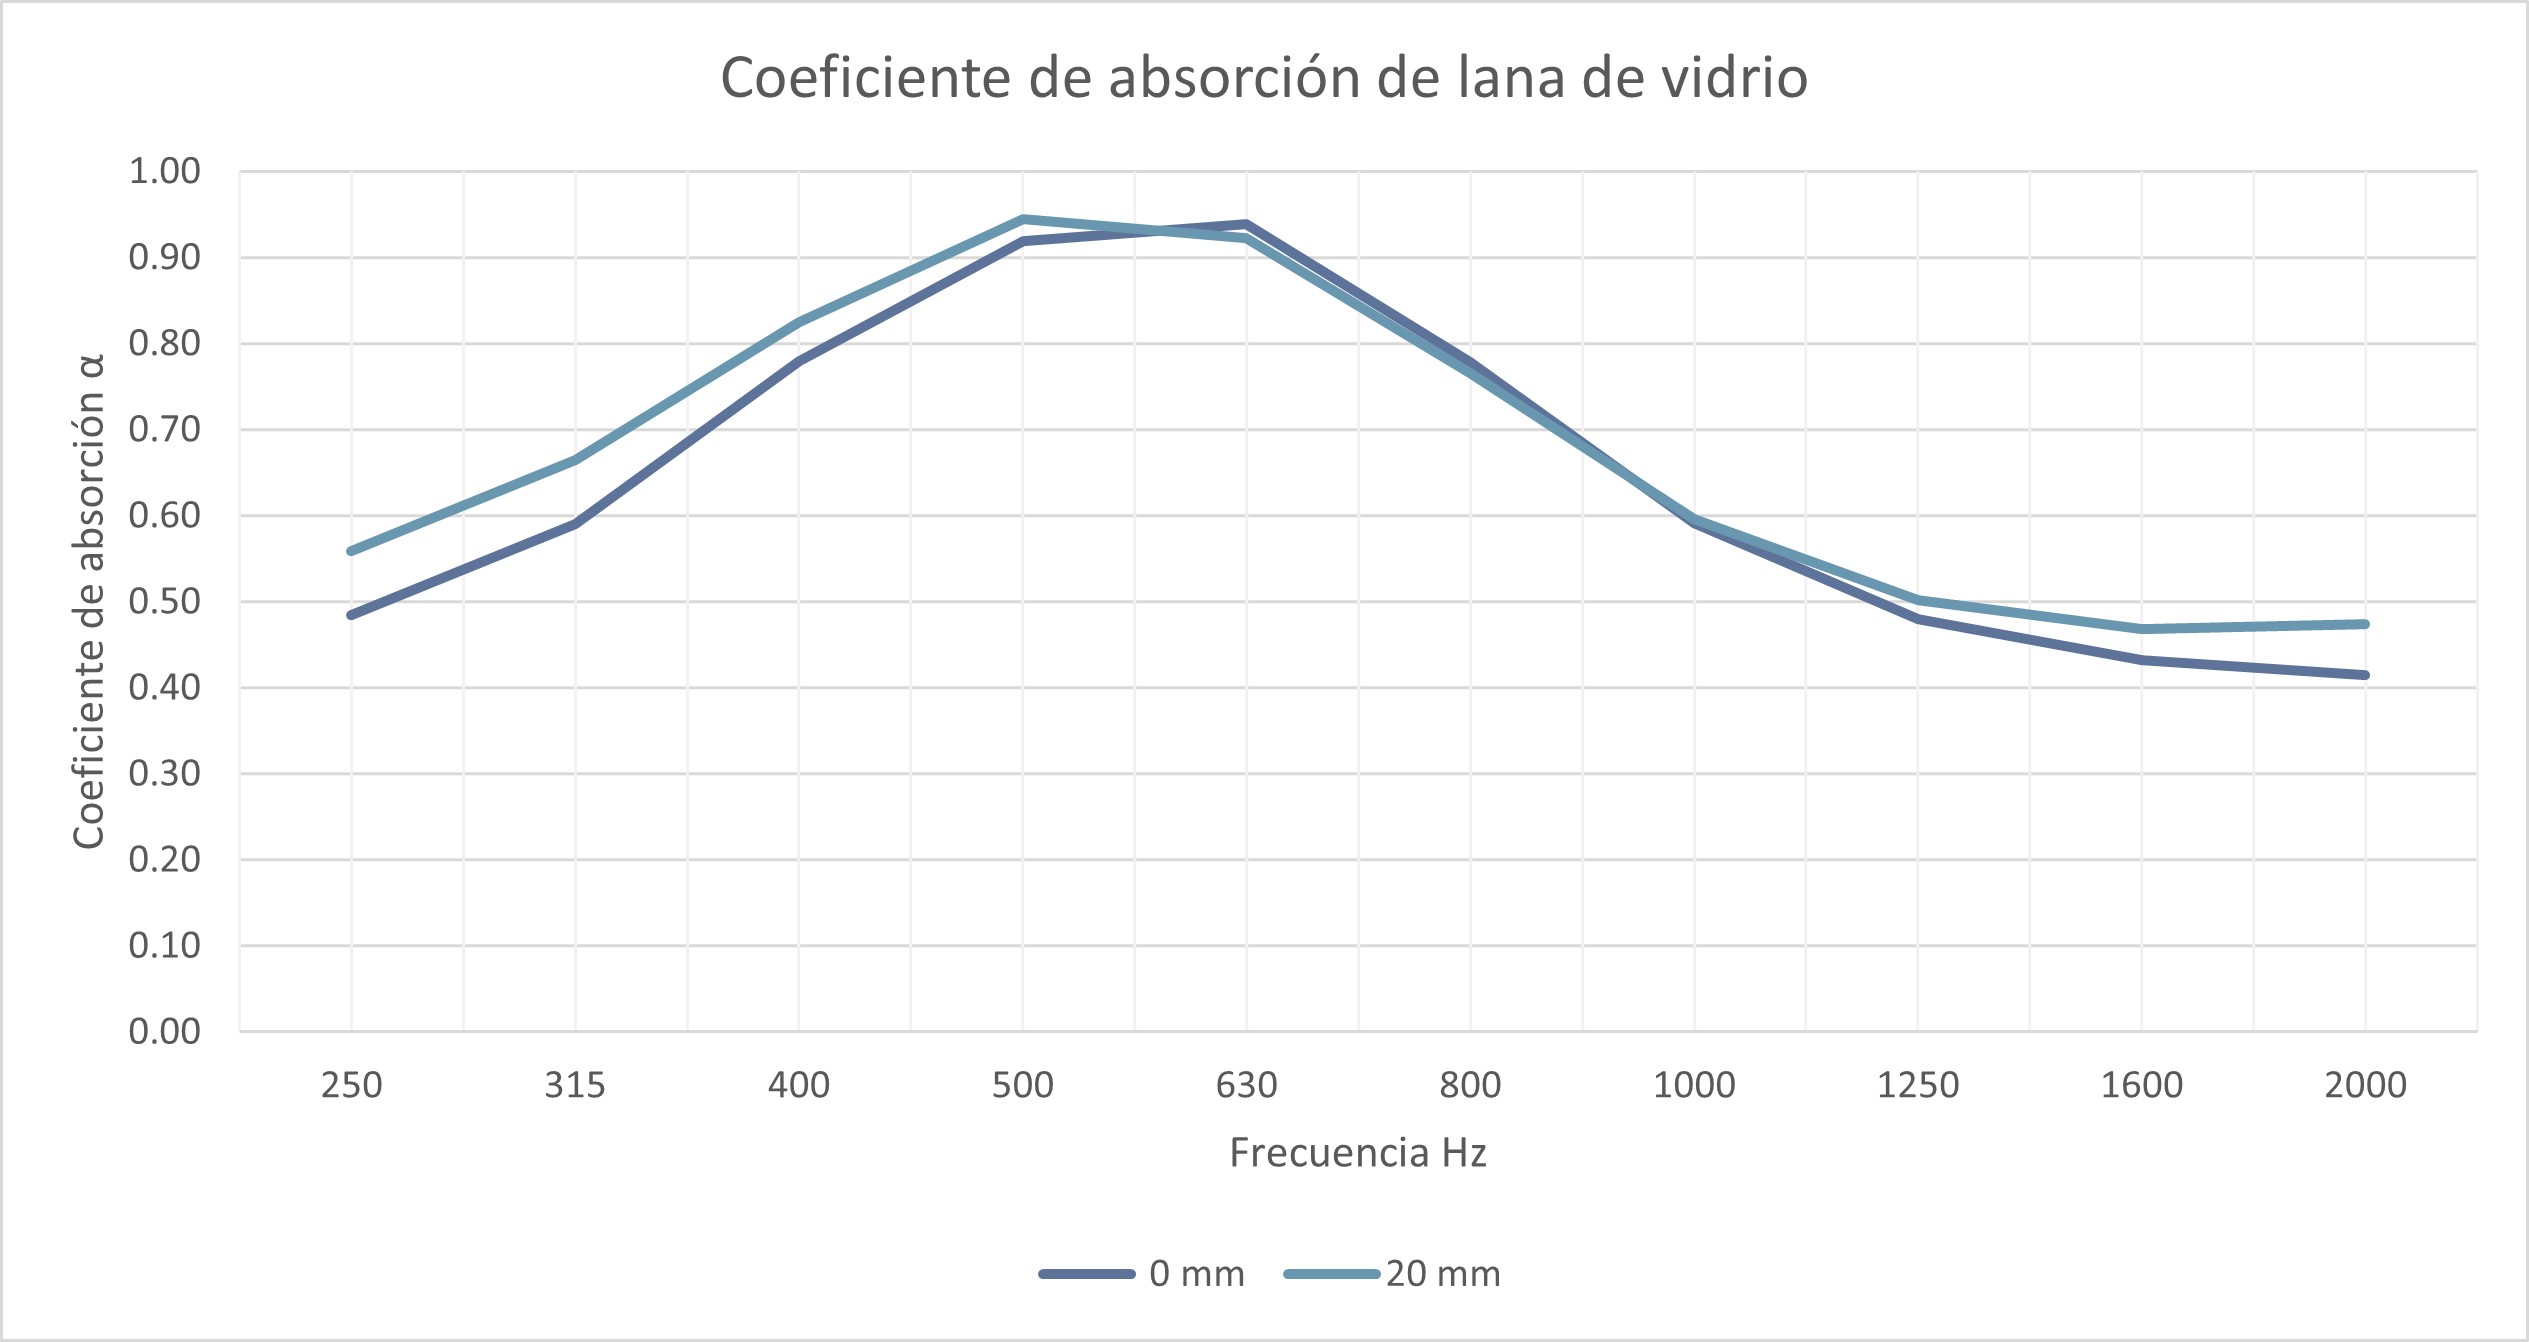
\includegraphics[width=10cm]{Imagenes/Medición abs/Grafico coef.abs LanaVidrio.png}
    \caption{Gráfico de coeficiente de absorción de madera ranurada con lana de vidrio con distinto plenum}
    \label{fig: grafico de coef abs de lana de vidrio}
\end{figure}

